% Modelo de Dissertação em Latex para o PPG em Engenharia Mecânica da UERJ
% Este modelo foi adaptado da versão disponibilizada no site da Engenharia Elétrica da UERJ
% http://www.pel.uerj.br/publico/Modelo_LaTeX_Dissertacao_UERJ.rar
% http://www.pel.uerj.br/defesas/
%
% Utilizei o WinEdt 6.0 com Miktex 2.9
%
% Para gerar o PDF usei a opção PDFTeXfy com o documento [masterthesis.tex] aberto e em foco.
%
% Não consegui usar as figuras em EPS como o modelo original. Usei PNG e JPG sem problemas.
%
% Felipe M. - 20/06/2012
%

% Modificações e adaptações ao modelo da UFPE feitas por João Cordeiro.
% Versão original disponibilizada como template do latex.
% Este modelo foi criado para servir de exemplo de formato, não devendo seu código ser
% utilizado como referência de formatação.
% PLAIN: O código é uma adaptação de uma adaptação. Funciona, mas está cheio de gambiarras.
%
% João Cordeiro - 05/03/2019
%



\documentclass[a4paper,12pt,oneside,openany,table,xcdraw]{uerj}

\usepackage[portuges]{babel}
%\usepackage[latin1]{inputenc}
\usepackage[utf8]{inputenc}
\usepackage{enumerate}
\usepackage{cite}
\usepackage{epsf,epsfig,psfig}
\usepackage{pagina}
\usepackage{indentfirst}
\usepackage{theorem}
\usepackage{fancyhdr}
\usepackage{setspace}
\usepackage{boxedminipage}
\usepackage{float}
\usepackage{makeidx}
\usepackage{amsmath}
\usepackage[hidelinks]{hyperref}
\usepackage{todonotes}
\usepackage{caption}
\usepackage{graphicx}
\usepackage{multirow}
\usepackage{blindtext}


\makeindex


\newtheorem{deff}{Definição}[section]
\numberwithin{equation}{chapter}

\theoremstyle{plain}

\bibliographystyle{abnt-num}

% Legenda (título) numerada via \caption --- sintaxe reservada do LaTeX --- seguida
% da fonte como texto comum. A fonte NÃO usa \caption*: não é uma legenda, e
% reaproveitar a sintaxe de legenda para texto livre gera ambiguidade.
\newcommand*{\captionsource}[3]{%
    \caption{\label{#1}#2.}%
    \par\vspace{-0.3cm}%
    {\centering\small Fonte: #3.\par}%
}


\begin{document}

\hypersetup{
    colorlinks,
    citecolor=black,
    filecolor=black,
    linkcolor=black,
    urlcolor=black,
    linktoc=all
}
% Infos do projeto
%

\newcommand{\thecenter}{Universidade Federal de Pernambuco}
\newcommand{\thedepartment}{Centro de Informática}
\newcommand{\thecourse}{Sistemas de Informação}
\newcommand{\thetitle}{Desenvolvimento de um Pipeline Analítico e Modelo de Otimização Multicritério para Alocação de Recursos na Gestão de Equipamentos Médico-Hospitalares}
\newcommand{\thetype}{Trabalho de Conclusão de Curso de Graduação}
\newcommand{\theproftitle}{Bacharel em Sistemas de Informação}
\newcommand{\thestudent}{Carlos Henrique da Silva Frey}
\newcommand{\theadvisor}{Profa. Maíra Araújo de Santana}
\newcommand{\thecity}{Recife}

% \thispagestyle{empty}\listoftodos\pagebreak
\thispagestyle{empty}\input{./01_Pre_textuais/Capa}
\pagebreak\thispagestyle{empty}\begin{center}

\thestudent

% \vfill
\vspace{2cm}

\textbf{\thetitle}

\vspace{6.0cm}

% \begin{figure}[hbt!]
% \begin{center}
% 
\includegraphics[width=10.48cm]{./01_Pre_textuais/logo_ufpe.png}
% \end{center}
% \end{figure}

\begin{flushright}
\parbox{8cm}{
\singlespacing{\begin{hyphenrules}{nohyphenation}
Monografia apresentada ao Curso de \thecourse, como requisito parcial para a obtenção do Título de \theproftitle, \thecenter.
\end{hyphenrules}
}
}

% \linebreak 
\vspace{2.0cm}
Orientador: \theadvisor\\
\end{flushright}


\par\vfill
%\vspace{2cm}

Recife\\2023

\end{center}
\pagebreak\thispagestyle{empty}$\!$\\
$\!$\\
$\!$\\
$\!$\\
$\!$\\
$\!$\\
$\!$\\
$\!$\\
$\!$\\
$\!$\\
$\!$\\
$\!$\\
$\!$\\
$\!$\\
$\!$\\
$\!$\\
$\!$\\
$\!$\\
$\!$\\
$\!$\\
$\!$\\
$\!$\\

\begin{flushright}
\textit{Qualquer tecnologia suficientemente}
\end{flushright}
\vspace{-1cm}
\begin{flushright}
\textit{avançada é indistinguível de magia.}
\end{flushright}
\begin{flushright}
Arthur C. Clarke
\end{flushright}

\thispagestyle{empty}
\pagebreak\thispagestyle{empty}\begin{center}
\textbf{RESUMO}
\end{center}

$\!$\\
\noindent
Este trabalho tem como objetivo... 

\vspace{1cm}

\hspace{-1.3cm}Palavras-chave: Palavra 1, Palavra 2, Palavra 3, Palavra 4. (4 a 6 palavras chave)
\pagebreak\thispagestyle{empty}\begin{center}
\textbf{ABSTRACT}
\end{center}

$\!$\\
\noindent
This work presents the development of an analytical pipeline integrated with a decision-support dashboard for the management of the technological assets of the Hospital das Clinicas of the Federal University of Pernambuco. The study addresses resource allocation under budget constraints, focusing on the replacement of obsolete medical equipment. The proposed methodology includes the automation of extraction, transformation, and loading stages to clean and consolidate operational data, followed by the definition of a failure-criticality prioritization index. Based on this index, the tool implements a budget-distribution utility that, given a financial cap set by the manager, automatically selects the set of equipment to replace, maximizing the aggregate impact of the investment under the budget constraint, thereby translating the multicriteria prioritization into an objective resource-allocation recommendation. Applied to real asset data, this utility turns the prioritized list into an actionable replacement plan, indicating not only \textit{which} equipment to prioritize but \textit{which} to actually replace given the available budget. The contribution is to provide the Clinical Engineering department with an analytical tool to support strategic resource allocation and improve the recovery of clinical service capacity.

\vspace{1cm}

\hspace{-1.3cm}Keywords: Clinical Engineering, ETL, Multicriteria optimization, Resource allocation, Medical equipment management.

\fancypagestyle{plain}{
\fancyhf{} % clear all header and footer fields
\renewcommand{\headrulewidth}{0pt}
\renewcommand{\footrulewidth}{0pt}}
\pagestyle{plain}

\pagebreak

\def\listfigurename{LISTA DE FIGURAS}\listoffigures
\def\listtablename{LISTA DE TABELAS}\listoftables
\newpage

\begin{center}
\textbf{LISTA DE SIGLAS}
\end{center}
$\!$\\

\begin{tabular}{lll}
$t_E$ & \hspace{1cm} & Tempo expiratório \\
$t_I$ & \hspace{1cm} & Tempo inspiratório \\
UFPE & \hspace{1cm} & Universidade Federal de Pernambuco \\
\end{tabular}    % não coloquei LISTA DE SIGLAS no meu trabalho, mas fica aqui a chamada comentada.
\def\contentsname{SUMÁRIO}\tableofcontents

\fancypagestyle{plain}{
\fancyhf{} % clear all header and footer fields
\fancyhead[R]{\thepage}
\setlength{\voffset}{-1cm}
\setlength{\headsep}{1cm}
\renewcommand{\headrulewidth}{0pt}
\renewcommand{\footrulewidth}{0pt}}

\pagestyle{plain}

\pagebreak
\chapter{Introdução}
\label{chapter:introducao}



\chapter{REFERENCIAL TEÓRICO}
\label{chap:refteorico}

\section{Engenharia clínica e gestão de tecnologia médico-hospitalar}

A engenharia clínica é o campo responsável por aplicar conhecimentos de
engenharia ao ambiente de saúde, com foco na gestão segura e eficiente das
tecnologias médico-hospitalares ao longo de todo o seu ciclo de vida --- da
aquisição ao descarte. A gestão de tecnologia médico-hospitalar (GTMH) abrange
atividades como incorporação, inventário, manutenção, controle de desempenho e
desativação dos equipamentos, com o objetivo de assegurar disponibilidade,
confiabilidade e segurança. No Brasil, o gerenciamento de tecnologias em saúde
nos estabelecimentos é objeto de regulamentação sanitária específica.

\todo[inline]{Cite aqui a regulamentação e a literatura de engenharia clínica que
você adotar (ex.: ANVISA RDC nº 509/2021; livros/artigos de GTMH). Insira no
formato ABNT.}

\section{Manutenção e ciclo de vida dos equipamentos}

As estratégias de manutenção costumam ser classificadas em corretiva (executada
após a falha), preventiva (programada para reduzir a probabilidade de falha) e
preditiva (baseada no monitoramento da condição do equipamento). O histórico de
manutenção corretiva, em particular, é um indicador relevante do estado de um
equipamento: o aumento da frequência e, sobretudo, do custo das intervenções
tende a acompanhar o envelhecimento do item, sinalizando a aproximação do fim de
sua vida útil econômica. O acompanhamento desses indicadores ao longo do tempo
fornece subsídios para decidir entre manter ou substituir um equipamento.

\todo[inline]{Inclua referências sobre tipos de manutenção e ciclo de vida/curva
de custos de equipamentos.}

\section{Criticidade e priorização de substituição}

Nem todos os equipamentos têm o mesmo impacto sobre a assistência. A criticidade
expressa a importância clínica e o risco associado a cada equipamento, sendo
usualmente representada em níveis (por exemplo, de baixa a alta). A priorização
de substituição busca ordenar os candidatos à troca combinando múltiplos
critérios --- tipicamente criticidade, idade e custo de manutenção ---, de modo
que os recursos, sempre limitados, sejam direcionados aos itens cuja renovação
traz maior retorno em segurança e em eficiência. Abordagens multicritério desse
tipo são amplamente empregadas no apoio à decisão em gestão de ativos e
fundamentam o modelo de otimização adotado neste trabalho.

\todo[inline]{Cite a literatura de priorização/análise multicritério aplicada à
substituição de equipamentos.}

\section{Integração de dados (ETL) e visualização da informação}

O paradigma ETL (\textit{Extract, Transform, Load}) descreve o processo de
extrair dados de fontes diversas, transformá-los para um formato consistente e
carregá-los em um destino de análise. Trata-se de uma abordagem fundamental
quando os dados de origem são heterogêneos, como ocorre com planilhas de
diferentes sistemas e épocas. Uma vez integrados, os dados podem ser explorados
por meio de painéis interativos (\textit{dashboards}), recurso característico de
soluções de \textit{Business Intelligence} (BI), que sintetizam grandes volumes
de informação em indicadores e visualizações de fácil leitura, favorecendo a
tomada de decisão baseada em dados.

\todo[inline]{Cite referências de ETL, BI e visualização de dados que embasarão
esta subseção.}


\chapter{MATERIAL E MÉTODO}
\label{chap:metodologia}

Este capítulo descreve a abordagem adotada para o desenvolvimento da ferramenta
de apoio à gestão de equipamentos médico-hospitalares e o método de tratamento
dos dados que sustenta os resultados apresentados no capítulo seguinte. Trata-se
de uma pesquisa aplicada, de natureza quantitativa e caráter exploratório,
conduzida na forma de desenvolvimento de software seguido de um estudo de caso
com dados reais do parque de equipamentos do HC-UFPE.

\section{Tecnologias e arquitetura da ferramenta}

A ferramenta foi implementada como uma aplicação \textit{desktop} em linguagem
Python (versão 3.12)~\cite{python312}, estruturada segundo o paradigma ETL. A
interface gráfica foi construída com a biblioteca PySide6 (\textit{bindings}
oficiais do \textit{framework} Qt 6)~\cite{pyside6}, enquanto a manipulação e o
tratamento dos dados utilizam a biblioteca pandas~\cite{pandas}. O gerenciamento
de dependências e o empacotamento do projeto são feitos com o
Poetry~\cite{poetry}, e a distribuição para o ambiente hospitalar (Windows) é
gerada como executável único por meio do PyInstaller~\cite{pyinstaller}.

A aplicação organiza-se em duas camadas principais: (i) uma camada de
transformação de dados, responsável por extrair, normalizar e cruzar as planilhas
de origem; e (ii) uma camada de apresentação, que calcula os indicadores e os
exibe em um painel interativo dividido em uma aba de Análise (gráficos e
indicadores) e uma aba de Dados (tabelas consultáveis). A separação entre
transformação e apresentação permite que a mesma base tratada alimente diferentes
visualizações de forma consistente. A \ref{fig:aba_dados} ilustra a aba de
Dados, na qual a base consolidada pode ser consultada em formato tabular.

\begin{figure}[H]
    \centering
    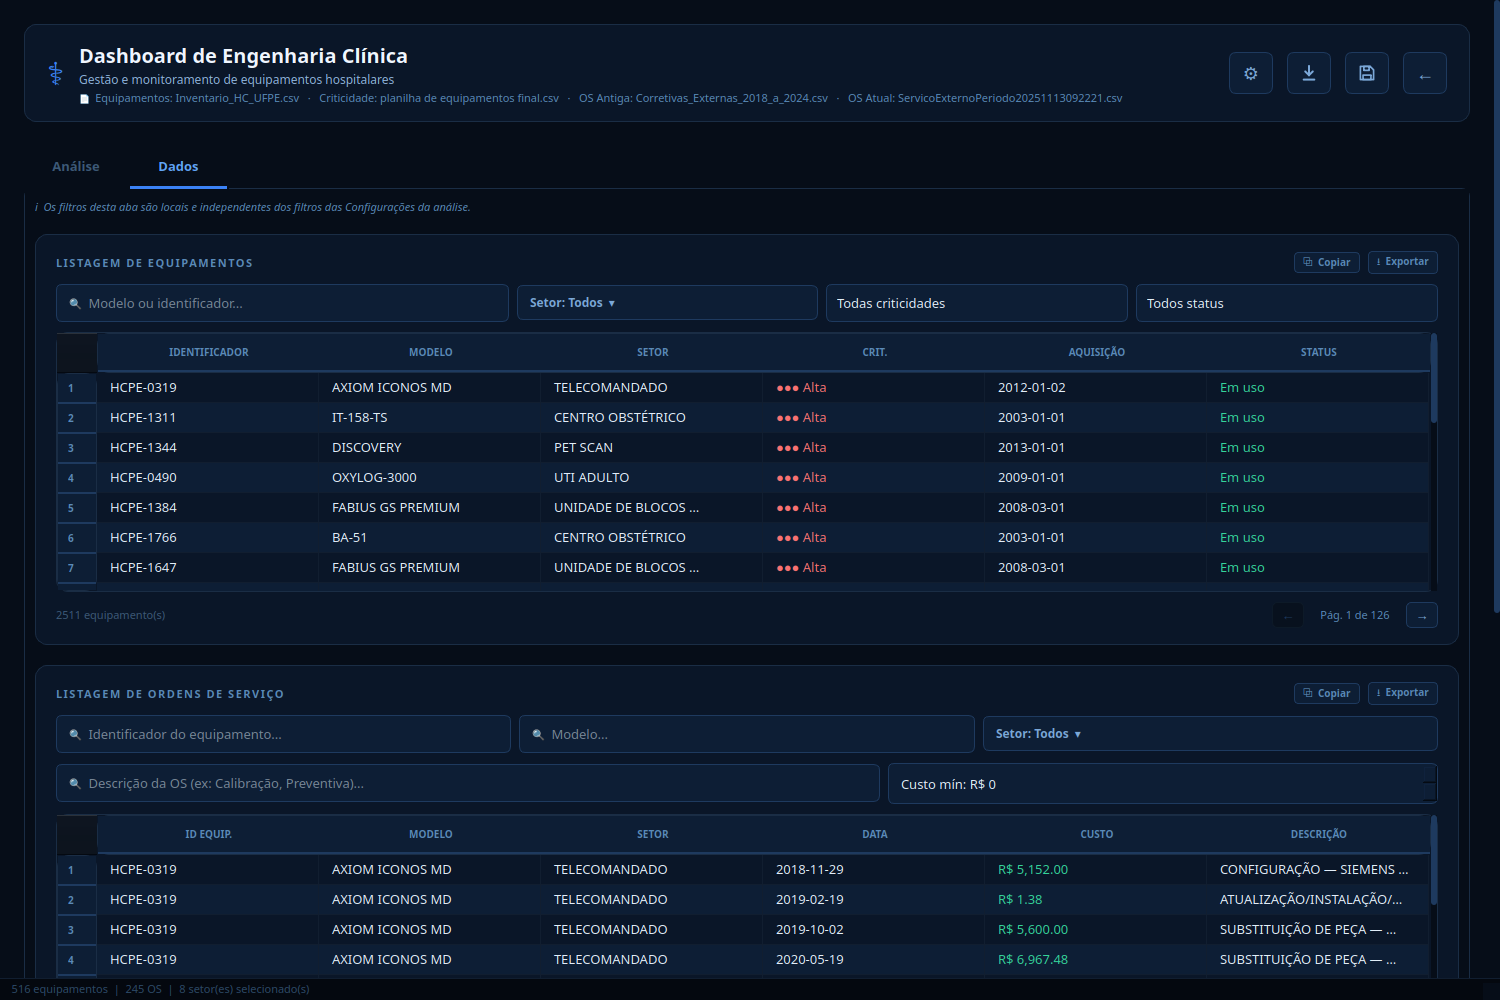
\includegraphics[width=\textwidth]{./imagens/04_aba_dados.png}
    \captionsource{fig:aba_dados}{Aba de Dados da ferramenta, com a base consolidada em formato tabular}{Elaborado pelo autor (2026)}
\end{figure}

\section{Fontes de dados}
\label{sec:fontes}

Foram utilizados quatro arquivos no formato CSV, fornecidos pela engenharia
clínica do HC-UFPE, organizados em quatro papéis distintos, conforme a
\ref{tab:fontes}.

\begin{table}[H]
    \centering
    \begin{tabular}{lp{9cm}}
        \hline
        \textbf{Insumo} & \textbf{Conteúdo} \\
        \hline
        Inventário & Cadastro dos equipamentos: identificador, modelo, localização (setor), data de aquisição e valor. \\
        Criticidade & Peso de criticidade por modelo de equipamento (escala de 1 a 3). \\
        OS --- formato antigo & Ordens de serviço corretivas no padrão legado, com datas e valores em convenção brasileira. \\
        OS --- formato atual & Ordens de serviço corretivas no padrão recente, com datas em formato ISO e valores em convenção norte-americana. \\
        \hline
    \end{tabular}
    \captionsource{tab:fontes}{Fontes de dados utilizadas e seus papéis}{Elaborado pelo autor (2026)}
\end{table}

A coexistência de dois formatos distintos de ordens de serviço --- resultado de
uma mudança no sistema de registro ao longo do tempo --- constitui um dos
principais desafios de integração tratados pela ferramenta, uma vez que cada
formato adota convenções diferentes de nomes de colunas, de representação de
datas e de separadores numéricos.

No estudo de caso conduzido neste trabalho, esses quatro papéis foram preenchidos
pelos arquivos reais do HC-UFPE listados na \ref{tab:arquivos}.

\begin{table}[H]
    \centering
    \begin{tabular}{ll}
        \hline
        \textbf{Insumo} & \textbf{Arquivo} \\
        \hline
        Inventário de equipamentos & \texttt{Inventario\_HC\_UFPE.csv} \\
        Criticidade & \texttt{planilha de equipamentos final.csv} \\
        OS --- formato antigo & \texttt{Corretivas\_Externas\_2018\_a\_2024.csv} \\
        OS --- formato atual & \texttt{ServicoExternoPeriodo20251113092221.csv} \\
        \hline
    \end{tabular}
    \captionsource{tab:arquivos}{Arquivos utilizados no estudo de caso do HC-UFPE}{Elaborado pelo autor (2026)}
\end{table}

\section{Processo de tratamento dos dados (ETL)}

\subsection*{Extração}

Cada arquivo CSV é lido tendo o ponto e vírgula como separador de campos. O
formato antigo de OS exige o descarte da primeira linha (cabeçalho duplicado), e
a planilha de criticidade possui o cabeçalho útil a partir da sexta linha, da
qual se aproveitam apenas as colunas de modelo e peso de criticidade.

\subsection*{Transformação e normalização}

A etapa central do processo é a unificação dos dois formatos de OS em um esquema
canônico único. Antes da concatenação, os valores são normalizados de acordo com
a sua origem, evitando ambiguidades de interpretação, conforme a
\ref{tab:normalizacao}.

\begin{table}[H]
    \centering
    \begin{tabular}{p{2.8cm}p{5cm}p{5cm}}
        \hline
        \textbf{Atributo} & \textbf{Formato antigo (BR)} & \textbf{Formato atual (ISO/US)} \\
        \hline
        Datas & dd/mm/aaaa (dia primeiro) & aaaa-mm-dd (ISO, sem ambiguidade) \\
        Valores monetários & ponto = milhar; vírgula = decimal & ponto = decimal \\
        Descrição do serviço & tipo de serviço + assistência & fornecedor \\
        \hline
    \end{tabular}
    \captionsource{tab:normalizacao}{Normalização dos atributos por formato de origem}{Elaborado pelo autor (2026)}
\end{table}

Em seguida, os nomes das colunas de ambos os formatos são mapeados para um
conjunto canônico (ordem de serviço, equipamento, data de abertura, data de
fechamento, serviço/assistência e identificador), e os registros são concatenados
em uma única base de ordens de serviço.

\subsection*{Carga e cruzamento (integração)}

A base unificada de OS é então cruzada com o inventário. Como as ordens de
serviço armazenam o identificador no padrão ``TAG,Patrimônio'' enquanto o
inventário utiliza apenas a TAG, ambos os lados são normalizados para a TAG
(porção anterior à primeira vírgula) antes do casamento --- procedimento que
evita a perda de uma parcela expressiva dos vínculos. Registros de OS sem
identificador são descartados para não corromper o custo atribuído aos demais
equipamentos. A criticidade é incorporada por meio da junção da planilha de pesos
com o inventário pelo nome do modelo; modelos sem correspondência recebem
criticidade mínima (nível 1). O custo de cada ordem de serviço é agregado por
equipamento, produzindo o custo total de manutenção corretiva de cada item. Ao
final, cada equipamento é representado por uma estrutura que reúne modelo, setor,
criticidade, data de aquisição, valor, custo acumulado e a lista de ordens de
serviço associadas, pronta para alimentar os indicadores do painel.

\section{Índice de priorização e modelo de otimização multicritério}
\label{sec:score}

Para apoiar a decisão de substituição, a ferramenta calcula um índice de
prioridade (\textit{score}) na escala de 0 a 100, combinando três critérios
complementares, conforme a \ref{tab:score}.

\begin{table}[H]
    \centering
    \begin{tabular}{lp{7cm}r}
        \hline
        \textbf{Critério} & \textbf{Regra} & \textbf{Pontuação máxima} \\
        \hline
        Idade & Equipamentos com 10 anos ou mais recebem a pontuação cheia & 20 pontos \\
        Criticidade & Proporcional ao nível de criticidade (nível $\div$ 3 $\times$ 50) & 50 pontos \\
        Custo de manutenção & Proporcional ao custo acumulado em relação ao maior custo do parque & 30 pontos \\
        \hline
    \end{tabular}
    \captionsource{tab:score}{Critérios e pontuações do índice de priorização}{Elaborado pelo autor (2026)}
\end{table}

A escolha desses três critérios --- criticidade, idade e custo de manutenção ---
alinha-se aos fatores recorrentemente adotados na literatura de priorização de
substituição de equipamentos médico-hospitalares~\cite{park2025evaluation,zamzam2021prioritisation}.
A pontuação de custo emprega uma normalização do tipo min-max, escalonando o custo
acumulado de cada item em relação ao maior custo do parque~\cite{sinsomboonthong2022performance}.

A criticidade é o critério de maior peso, refletindo a prioridade clínica do
equipamento; a idade e o custo histórico de manutenção complementam a avaliação,
capturando, respectivamente, o envelhecimento e o ônus financeiro acumulado. O
painel permite ajustar interativamente tanto os pesos de cada critério quanto o
limite de idade considerado, recalculando o ranking em tempo real --- o que
confere à ferramenta um caráter exploratório e adaptável a diferentes políticas
de gestão.

A partir desse índice, a ferramenta materializa um modelo de otimização
multicritério para a alocação do orçamento de substituição. Dado um orçamento
disponível, informado pelo gestor, a funcionalidade de distribuição de orçamento
percorre os equipamentos em ordem decrescente de prioridade e seleciona aqueles
cuja substituição cabe no recurso disponível, de modo a maximizar o impacto
agregado em segurança e em redução de custo. Dessa forma, o \textit{score} deixa
de ser apenas um ranking e passa a orientar objetivamente \textit{quais}
equipamentos substituir diante de uma restrição orçamentária --- traduzindo a
priorização multicritério em uma recomendação de alocação de recursos.

\section{Recorte de análise e indicadores gerados}

Por padrão, a ferramenta aplica um recorte sobre os setores de maior criticidade
assistencial (UTI Adulto, UTI Neonatal, Bloco Cirúrgico e Centro Obstétrico),
seleção que pode ser ampliada ou alterada pelo usuário no menu de configurações.
Sobre o conjunto filtrado, são calculados os seguintes indicadores: total de
equipamentos, total de ordens de serviço e gasto total (KPIs); distribuição
etária do parque; ranking de prioridade de substituição; histórico mensal e anual
de emissão de OS; evolução do custo por ano; custo por setor; e os equipamentos
de maior custo acumulado. Todos os indicadores reagem dinamicamente aos filtros
aplicados.

\section{Procedimento de execução e validação}

O fluxo de uso parte de uma tela de importação, na qual o usuário seleciona as
quatro planilhas. Após o processamento --- executado em segundo plano para
preservar a responsividade da interface --- é exibida uma pré-visualização da
base de OS consolidada para conferência antes da confirmação. Confirmada, a
aplicação apresenta o painel de análise. As seleções de arquivos e as
configurações de análise podem ser salvas e recarregadas, garantindo a
reprodutibilidade dos estudos. Os resultados reportados no capítulo seguinte foram
obtidos exatamente por esse procedimento, carregando-se as quatro planilhas reais
do HC-UFPE e processando-as com a ferramenta.


\chapter{RESULTADOS E DISCUSSÃO}

Os resultados apresentados neste capítulo foram obtidos a partir da execução
real do software desenvolvido (\texttt{poetry run dashboard}), com as quatro
planilhas de origem carregadas e a análise processada. As figuras referenciadas
encontram-se no diretório \texttt{imagens/}.

\section{Configuração da análise}

A Tabela~\ref{tab:insumos} relaciona os insumos utilizados na análise. O sistema
consolida o inventário e a criticidade dos equipamentos com as ordens de serviço
(OS) provenientes de dois formatos distintos de planilha: o formato antigo e o
formato atual.

\begin{table}[H]
    \centering
    \captionsource{tab:insumos}{Insumos utilizados na análise}{Elaborado pelo autor (2026)}
    \begin{tabular}{ll}
        \hline
        \textbf{Insumo} & \textbf{Arquivo} \\
        \hline
        Inventário de equipamentos & \texttt{Inventario\_HC\_UFPE.csv} \\
        Criticidade & \texttt{planilha de equipamentos final.csv} \\
        OS --- formato antigo & \texttt{Corretivas\_Externas\_2018\_a\_2024.csv} \\
        OS --- formato atual & \texttt{ServicoExternoPeriodo20251113092221.csv} \\
        \hline
    \end{tabular}
\end{table}

A base processada compreende:

\begin{itemize}
    \item \textbf{Inventário total processado:} 2.511 equipamentos.
    \item \textbf{Ordens de serviço consolidadas (base bruta):} 2.883 OS
    (2.568 do formato antigo e 318 do atual).
    \item \textbf{Recorte de análise (filtro de setores críticos --- padrão do
    sistema):} 8 sub-setores de UTI Adulto, UTI Neonatal, Bloco Cirúrgico e
    Centro Obstétrico, totalizando 516 equipamentos.
\end{itemize}

Todos os indicadores a seguir referem-se ao recorte de 516 equipamentos dos
setores críticos.

\section{Indicadores principais (KPIs)}

A Tabela~\ref{tab:kpis} sintetiza os principais indicadores de desempenho do
recorte analisado.

\begin{table}[H]
    \centering
    \captionsource{tab:kpis}{Indicadores principais (KPIs) dos setores críticos}{Elaborado pelo autor (2026)}
    \begin{tabular}{lr}
        \hline
        \textbf{Indicador} & \textbf{Valor} \\
        \hline
        Total de equipamentos (setores críticos) & 516 \\
        Total de OS emitidas & 245 \\
        Gasto total em OS & R\$~315.613,59 \\
        Custo médio por OS & $\approx$ R\$~1.288 \\
        Idade média do parque & 7,3 anos \\
        Equipamentos com $\geq$ 10 anos & 97 (18,8\%) \\
        \hline
    \end{tabular}
\end{table}

Quanto à composição por criticidade, o recorte distribui-se em: Alta (3) = 134
equipamentos; Média (2) = 156; e Baixa (1) = 226. Em relação ao status, 100\%
constam como ``Em uso'', uma vez que a base não traz equipamentos baixados ou
inoperantes nesse recorte. A Figura~\ref{fig:aba_analise} apresenta a aba de
análise do dashboard.

\begin{figure}[H]
    \centering
    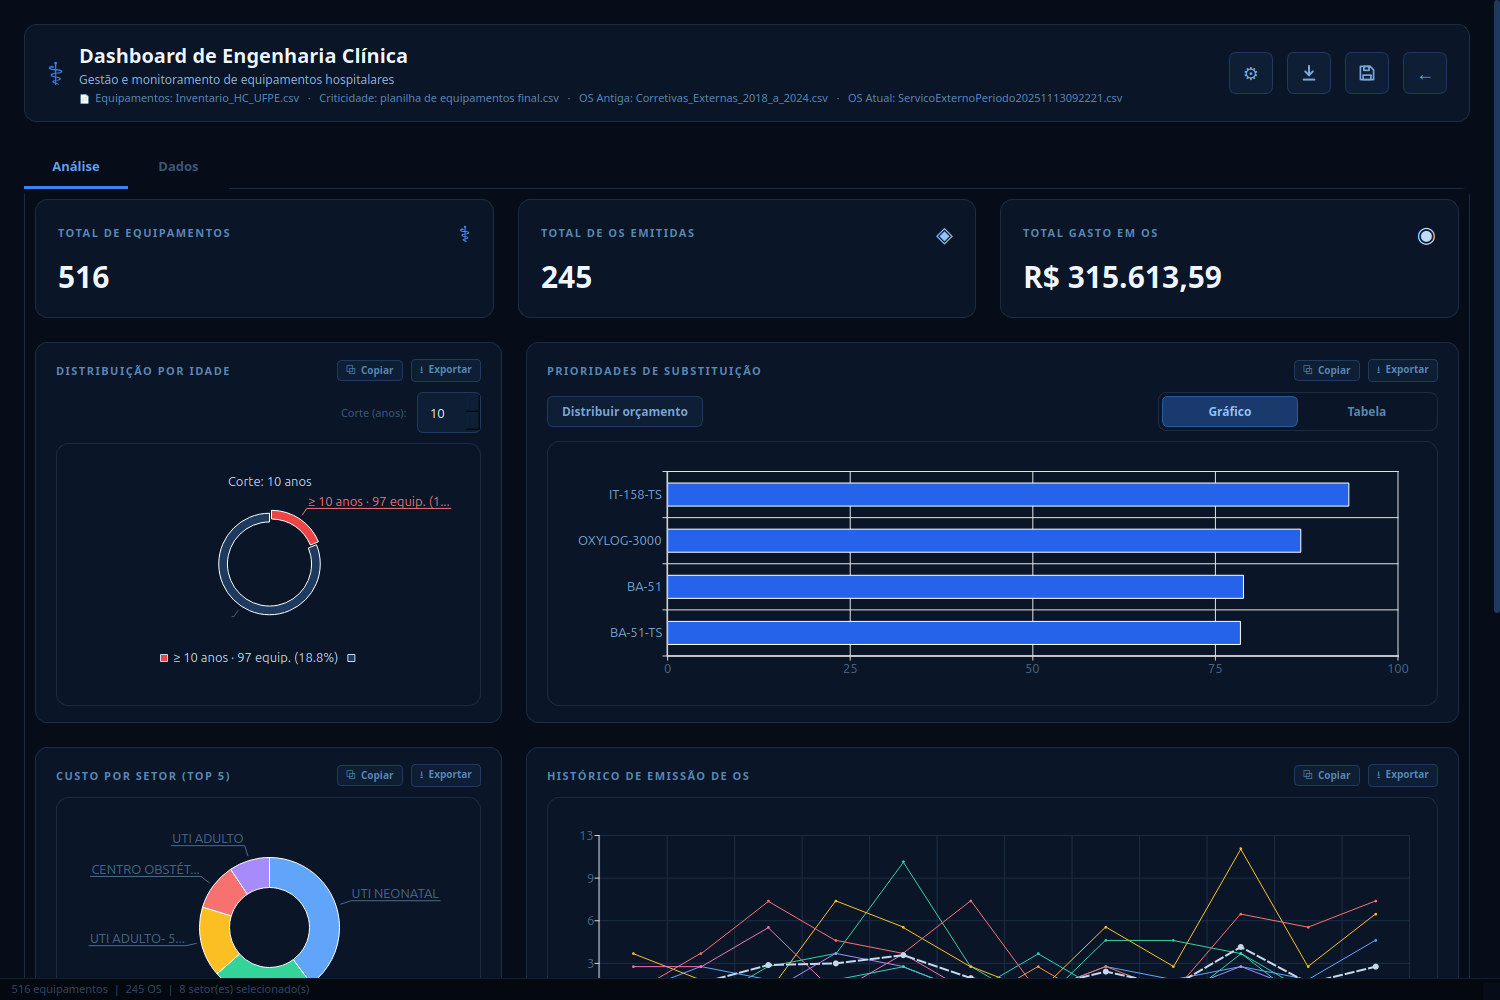
\includegraphics[width=\textwidth]{./imagens/01_aba_analise.png}
    \captionsource{fig:aba_analise}{Aba de análise do dashboard}{Elaborado pelo autor (2026)}
\end{figure}

\section{Distribuição por idade}

Dos 516 equipamentos, 97 (18,8\%) já ultrapassaram o corte de 10 anos de vida
útil. A idade média (7,3 anos) é puxada para baixo por aquisições recentes, mas
há uma cauda relevante de equipamentos antigos --- de até 23 anos ---, justamente
os de maior criticidade.

\section{Prioridade de substituição}

O \textit{score} (0--100) combina idade, criticidade e custo acumulado de
manutenção. A Tabela~\ref{tab:ranking} apresenta o topo do ranking de prioridade
de substituição.

\begin{table}[H]
    \centering
    \captionsource{tab:ranking}{Topo do ranking de prioridade de substituição}{Elaborado pelo autor (2026)}
    \begin{tabular}{clllccr}
        \hline
        \textbf{\#} & \textbf{Identificador} & \textbf{Modelo} & \textbf{Setor} & \textbf{Crit.} & \textbf{Idade} & \textbf{Score} \\
        \hline
        1 & HCPE-1311 & IT-158-TS & Centro Obstétrico & 3 & 23 & 100,0 \\
        2 & HCPE-0490 & OXYLOG-3000 & UTI Adulto & 3 & 17 & 93,3 \\
        3 & HCPE-1766 & BA-51 & Centro Obstétrico & 3 & 23 & 86,7 \\
        4 & HCPE-1220 & BA-51 & UTI Neonatal & 3 & 23 & 78,8 \\
        5 & HCPE-1256 & BA-51-TS & UTI Neonatal & 3 & 23 & 78,4 \\
        6 & HCPE-2667 & DX-3012 & UTI Adulto 5º & 3 & 14 & 74,9 \\
        7 & HCPE-0547 & BILITRON-3006-BTP & UTI Neonatal & 3 & 13 & 72,5 \\
        8 & HCPE-0549 & BILITRON-3006-BTP & UTI Neonatal & 3 & 13 & 72,2 \\
        \hline
    \end{tabular}
\end{table}

O topo do ranking é dominado por equipamentos de criticidade máxima (3) e idade
$\geq$ 13 anos, concentrados em UTI Neonatal e Centro Obstétrico (incubadoras e
aquecedores BA-51, fototerapia BILITRON, ventilador de transporte OXYLOG).

\section{Histórico de emissão de OS e custo por ano}

A Tabela~\ref{tab:historico} apresenta a evolução anual do número de OS, do custo
total e do custo médio por OS.

\begin{table}[H]
    \centering
    \captionsource{tab:historico}{Histórico de emissão de OS e custo por ano}{Elaborado pelo autor (2026)}
    \begin{tabular}{lrrr}
        \hline
        \textbf{Ano} & \textbf{OS} & \textbf{Custo total} & \textbf{Custo médio/OS} \\
        \hline
        2018 & 36 & R\$~47.377,68 & R\$~1.316 \\
        2019 & 23 & R\$~16.690,74 & R\$~726 \\
        2020 & 56 & R\$~30.341,51 & R\$~542 \\
        2021 & 56 & R\$~21.040,99 & R\$~376 \\
        2022 & 23 & R\$~6.431,00 & R\$~280 \\
        2023 & 21 & R\$~38.613,70 & R\$~1.839 \\
        2024 & 19 & R\$~76.557,06 & R\$~4.029 \\
        2025\textsuperscript{*} & 11 & R\$~78.560,91 & R\$~7.142 \\
        \hline
    \end{tabular}
\end{table}

\noindent \textsuperscript{*} 2025 é ano parcial (dados até 13/11/2025).

\begin{figure}[H]
    \centering
    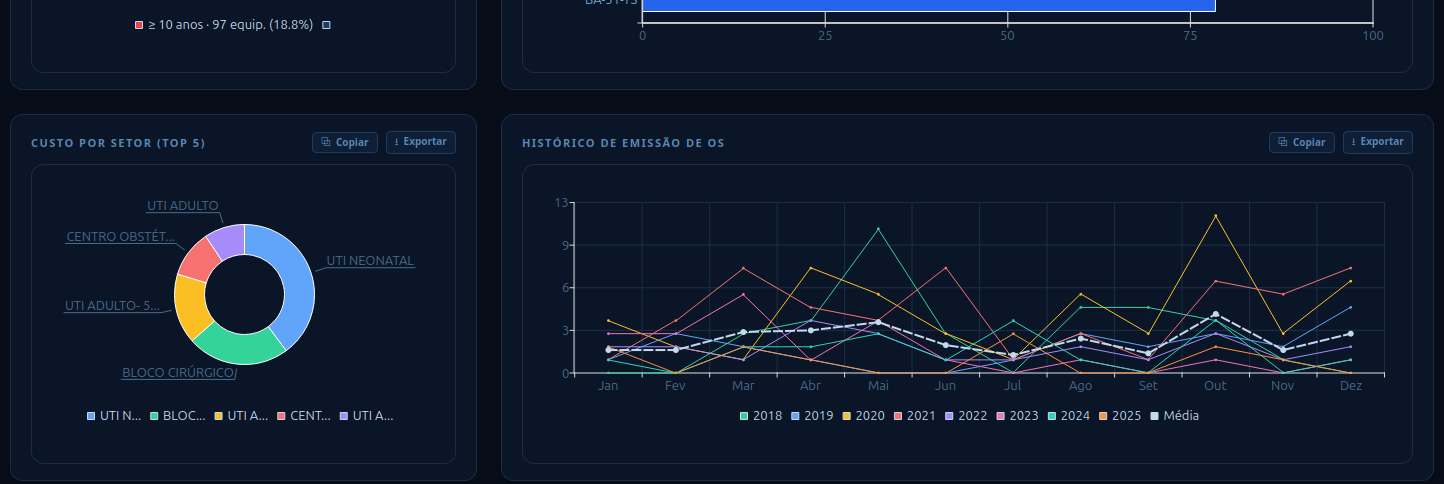
\includegraphics[width=\textwidth]{./imagens/02_custo_setor_historico_os.png}
    \captionsource{fig:custo_setor}{Custo por setor e histórico de OS}{Elaborado pelo autor (2026)}
\end{figure}

\begin{figure}[H]
    \centering
    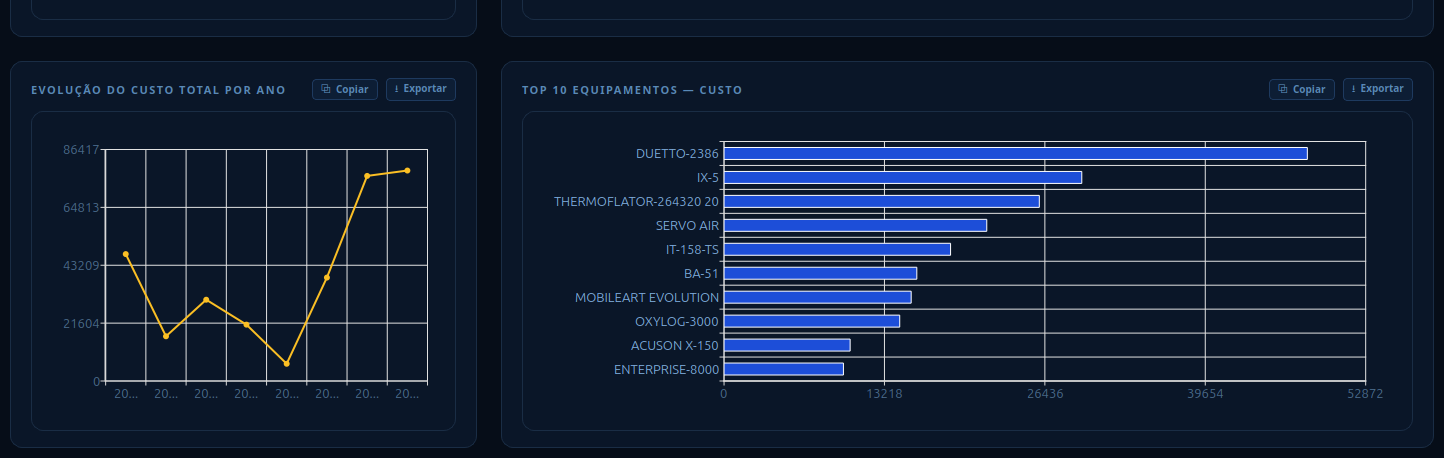
\includegraphics[width=\textwidth]{./imagens/03_evolucao_custo_top10.png}
    \captionsource{fig:evolucao_custo}{Evolução do custo e Top 10 equipamentos}{Elaborado pelo autor (2026)}
\end{figure}

\section{Concentração de custo por setor}

A Tabela~\ref{tab:custo_setor} evidencia a concentração do gasto corretivo por
setor.

\begin{table}[H]
    \centering
    \captionsource{tab:custo_setor}{Concentração de custo em OS por setor}{Elaborado pelo autor (2026)}
    \begin{tabular}{lrr}
        \hline
        \textbf{Setor} & \textbf{Custo em OS} & \textbf{Equip.} \\
        \hline
        UTI Neonatal & R\$~121.888,44 & 211 \\
        Bloco Cirúrgico & R\$~72.207,74 & 111 \\
        UTI Adulto 5º andar & R\$~49.639,32 & 61 \\
        Centro Obstétrico & R\$~33.444,51 & 91 \\
        UTI Adulto & R\$~28.595,79 & 24 \\
        UTI Adulto / URCC & R\$~9.837,79 & 1 \\
        \hline
    \end{tabular}
\end{table}

A UTI Neonatal, sozinha, responde por $\sim$39\% de todo o gasto corretivo do
recorte.

\section{Top 10 equipamentos por custo}

Agrupados por modelo, os dez equipamentos de maior custo são: DUETTO-2386 e IX-5
(incubadoras), THERMOFLATOR-264320 e SERVO AIR (ventilação), IT-158-TS, BA-51,
MOBILEART EVOLUTION, OXYLOG-3000, ACUSON X-150 e ENTERPRISE-8000. Predominam,
portanto, equipamentos de suporte à vida neonatal e de ventilação.

\section{Interpretação dos resultados}

\subsection{O custo de manutenção está migrando de ``muitas OS baratas'' para ``poucas OS caras''}

Entre 2020 e 2022, o parque gerava muitas ordens de baixo valor, com o custo
médio caindo até $\approx$ R\$~280/OS em 2022. A partir de 2023, o padrão se
inverte: o número de OS cai (de 56 para cerca de 11--21 por ano), mas o custo
médio por OS dispara --- de R\$~280 (2022) para R\$~4.029 (2024) e R\$~7.142
(2025). Esse é o comportamento típico de um parque envelhecendo: falhas mais
graves, peças mais caras e intervenções de maior porte. Mesmo com 2025 ainda
parcial, o gasto anual já supera o de 2024.

\subsection{Risco e custo estão concentrados nos mesmos setores}

A UTI Neonatal lidera o gasto corretivo ($\sim$39\% do total) e também concentra
os equipamentos do topo do ranking de substituição (BA-51, BILITRON, IX-5). Não
se trata de dispersão: há um núcleo crítico onde criticidade alta, idade elevada
e custo de manutenção coincidem --- exatamente o alvo no qual a substituição traz
maior retorno em segurança do paciente e redução de custo.

\subsection{Há uma cauda de equipamentos no fim da vida útil}

18,8\% do parque crítico já passou de 10 anos, e o topo do ranking chega a 23
anos de uso em equipamentos de criticidade 3. São candidatos diretos a
substituição planejada --- o software materializa isso no \textit{score} e na
funcionalidade ``Distribuir orçamento''.

\subsection{Valor da ferramenta para a gestão}

O dashboard converte cerca de 2.900 OS, dispersas em dois formatos de planilha,
em indicadores acionáveis: prioriza substituições por evidência (idade +
criticidade + custo), localiza onde o dinheiro está sendo gasto (UTI Neonatal) e
expõe a tendência de custo crescente --- insumos diretos para justificar
investimento em renovação de parque na engenharia clínica do HC-UFPE.

\subsection{Limitações}

O ano de 2025 é parcial; todos os equipamentos constam como ``Em uso'' (a base
não registra baixas); e os valores refletem apenas manutenção corretiva externa
do recorte escolhido (UTI, Bloco Cirúrgico e Centro Obstétrico). Trocar as
planilhas de OS (por exemplo, incluindo corretivas internas) ou ampliar os
setores no menu de configurações altera os números --- o que reforça o caráter
exploratório da ferramenta.



% inserir demais capítulos aqui
% -----------------------------
% -----------------------------
% -----------------------------
% -----------------------------





\pagebreak
\chapter{CONCLUSÃO}
\label{chapter:conclusao}

%breve resumo do que foi feito
%pontos de destaque dos resultados
%desafios
%perspectivas futuras



\pagebreak
\def\bibname{REFERÊNCIAS}




% abaixo segue a chamada para o arquivo [.BIB]. Utilizei o programa JABREF para montar o arquivo com minhas referências.
% \bibliography{dissertacao}
%\bibliography{tcc}
\bibliography{referenciasTCC}




%felipe% \printindex    %Removi o índice remissivo para a versão oficial do trabalho.


\end{document}